% !TEX root = Entwurf_goApp.tex
\section{Sequenzdiagramme}

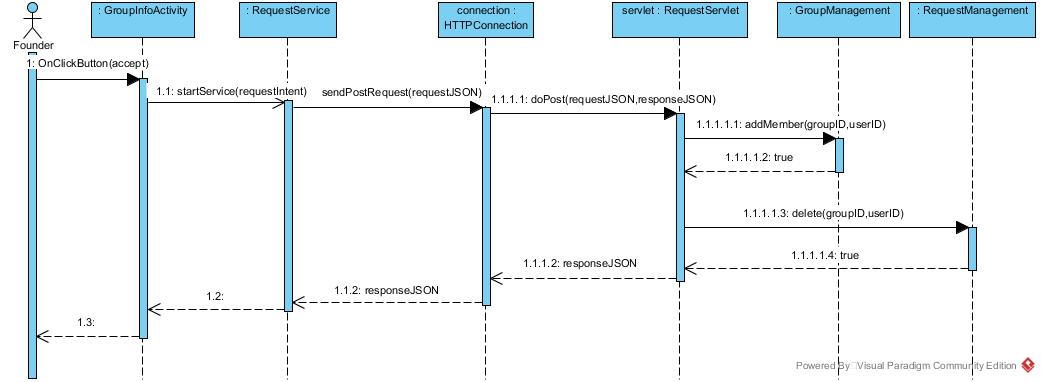
\includegraphics[width=1.1\textwidth]{addMemberSequenceDiagram.jpg}

\subsubsection{Activity-Service Kommunikation}
	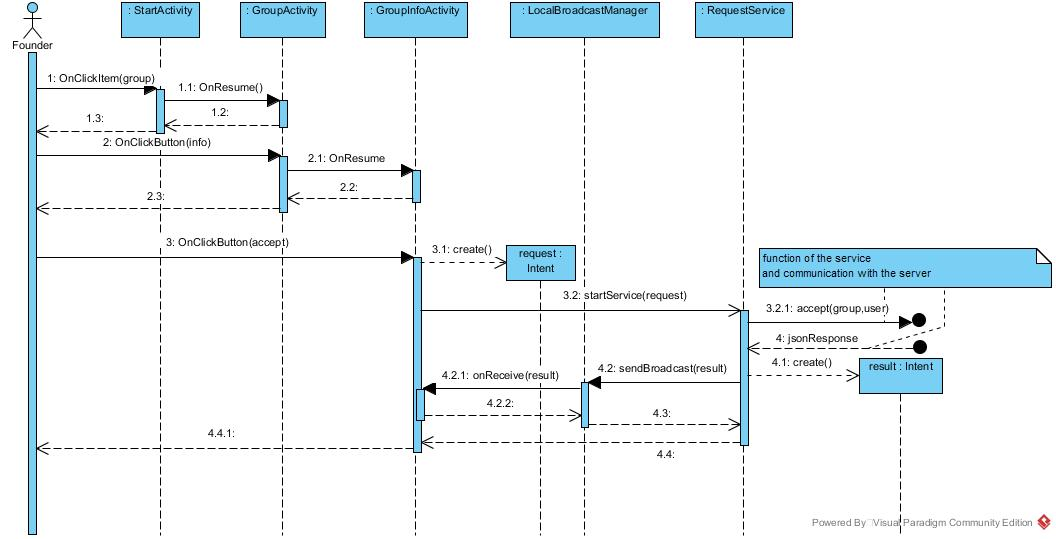
\includegraphics[width=1.1\textwidth]{Activity_Service.jpg}
	
\subsubsection{Service-ServerConnection Kommunikation}
Wenn bei dem RequestService die accept Methode aufgerufen wird, erstellt dieser zunächst ein JSONObject, in dem die Serveranfrage codiert wird. Er fügt dem JSONObject
\begin{itemize}
\item  die ID der Anfrage,
\item den Namen der Methode, welche auf dem Servlet aufgerufen werden soll,
\item die ID der Gruppe, zu der die Gruppenanfrage gehört und
\item die ID des Users welcher in die Gruppe aufgenommen werden will hinzu.
Zusätzlich erstellt der Service eine HTTPConnection und übergibt ihr den Namen des Servlets, an welches die Anfrage geschickt werden soll.
Danach holt er sich von dem JSONObject den JSON-String, in dem die zuvor hinzugefügten Daten enthalten sind. Den übergibt er der Methode sendPostRequest des Klasse HTTPConnection.
Diese sendet dann die Anfrage an den Server, welcher die Anfrage bearbeitet (\hypertarget{ServletDatenbank}{siehe Servlet-Datenbankmanagement Kommunikation}). Der Server sendet ein JSON-String als Antwort zurück, aus welchem die sendPostRequest-Methode ein JSONObject erzeugt und dieses an den RequestService zurück gibt.
%TODO brauchen wir AnfrageID überhaupt
\end{itemize}
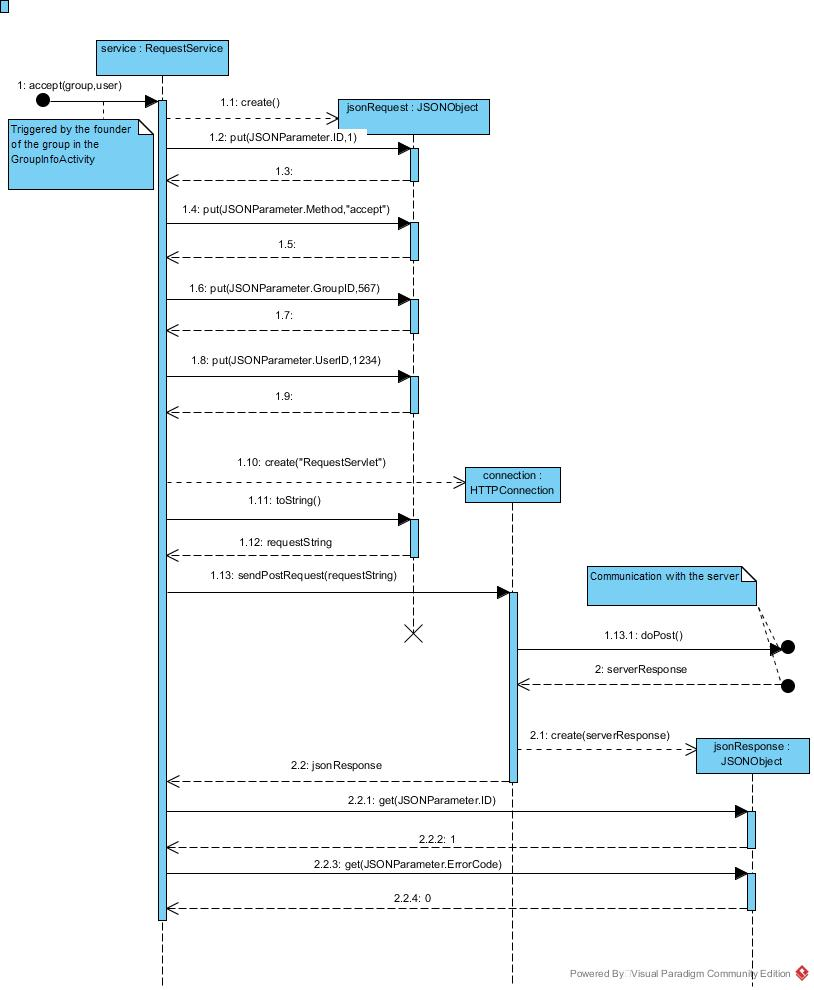
\includegraphics[width=1.1\textwidth]{Service_ServerConnection.jpg}

\hyperlink{ServletDatenbank}
\subsubsection{Servlet-Datenbankmanagement Kommunikation}
\includegraphics[width=1.1\textwidth]{Servlet_MAnagement.jpg}

\subsubsection{Clustering Algorithmus}
	
	\newpage